\documentclass[a4paper, 11pt]{article}
\usepackage[UTF8, scheme = plain]{ctex}
\usepackage{xcolor}     %高亮使用的颜色
\usepackage{amsmath}
\usepackage{graphicx}
\usepackage{geometry}
\usepackage{listings}
\geometry{scale=0.8}
\linespread{1.5}
\usepackage{hyperref}

\title{	
\normalfont \normalsize
\textsc{School of Data and Computer Science, Sun Yat-sen University} \\ [25pt] %textsc small capital letters
\rule{\textwidth}{0.5pt} \\[0.4cm] % Thin top horizontal rule
\huge  E05 Family Problem ( Prolog )\\ % The assignment title
\rule{\textwidth}{2pt} \\[0.5cm] % Thick bottom horizontal rule
\author{20214966 Yangkai Lin 20214810 Suixin Ou}
\date{\normalsize\today}
}

\begin{document}
\maketitle
\tableofcontents
\newpage
\section{About Cousin and Removed}
\textbf{What Is a First Cousin, Twice Removed?}

If someone walked up to you and said, ``Howdy, I'm your third cousin, twice removed," would you have any idea what they meant? Most people have a good understanding of basic relationship words such as ``mother," ``father," ``aunt," ``uncle," ``brother," and ``sister." But what about the relationship terms that we don't use in everyday speech? Terms like ``second cousin" and ``first cousin, once removed"? We don't tend to speak about our relationships in such exact terms (``cousin" seems good enough when you are introducing one person to another), so most of us aren't familiar with what these words mean.

\textbf{Relationship Terms}

Sometimes, especially when working on your family history, it's handy to know how to describe your family relationships more exactly. The definitions below should help you out.

\textbf{Cousin (a.k.a ``first cousin")}

Your first cousins are the people in your family who have two of the same grandparents as you. In other words, they are the children of your aunts and uncles.

\textbf{Second Cousin}

Your second cousins are the people in your family who have the same great-grandparents as you., but not the same grandparents.

\textbf{Third, Fourth, and Fifth Cousins}

Your third cousins have the same great great grandparents, fourth cousins have the same great-great-great-grandparents, and so on.

\textbf{Removed}

When the word ``removed" is used to describe a relationship, it indicates that the two people are from different generations. You and your first cousins are in the same generation (two generations younger than your grandparents), so the word ``removed" is not used to describe your relationship.

The words ``\textbf{once removed}" mean that there is a difference of one generation. For example, your mother's first cousin is your first cousin, once removed. This is because your mother's first cousin is one generation younger than your grandparents and you are two generations younger than your grandparents. This one-generation difference equals ``once removed."

\textbf{Twice removed} means that there is a two-generation difference. You are two generations younger than a first cousin of your grandmother, so you and your grandmother's first cousin are first cousins, twice removed.
\section{Problem Description}
Please fulfill the following tasks by using \texttt{Prolog}:
\begin{enumerate}
\item Using the predicates \textbf{male}, \textbf{female}, \textbf{child}, and \textbf{spouse}, write facts and rules describing the family tree in Figure \ref{fig:family}, and add the fact that William has a daughter Charlotte. Please do not write redundant facts that can be defined with rules.

\item Write rules describing the predicates \textbf{Grandchild}, \textbf{Greatgrandparent}, \textbf{Ancestor}, \textbf{Sibling}, \textbf{Brother}, \textbf{Sister}, \textbf{Daughter}, \textbf{Son}, \textbf{FirstCousin}, \textbf{BrotherInLaw}, \textbf{SisterInLaw}, \textbf{Aunt}, and \textbf{Uncle}.

\item Find out the proper definition of \textbf{\emph{m}th cousin \emph{n} times removed}, and write rules to define the predicate \texttt{mthCousinNremoved(X,Y,M,N)}. \emph{Hint: You'd better define a helper predicate \texttt{distance(X,Y,N)} meaning that there are N generations between X and Y by recursion ( please refer to \texttt{hanoi.pl}).}

\item ASK who are \textbf{Elizabeth’s grandchildren}, \textbf{Diana’s brothers-in-law}, \textbf{Zara’s great-grandparents}, \textbf{Eugenie’s ancestors}, and \textbf{Charlotte’s first cousin once removed}.
\end{enumerate}

\begin{figure}[h]  
  \centering
  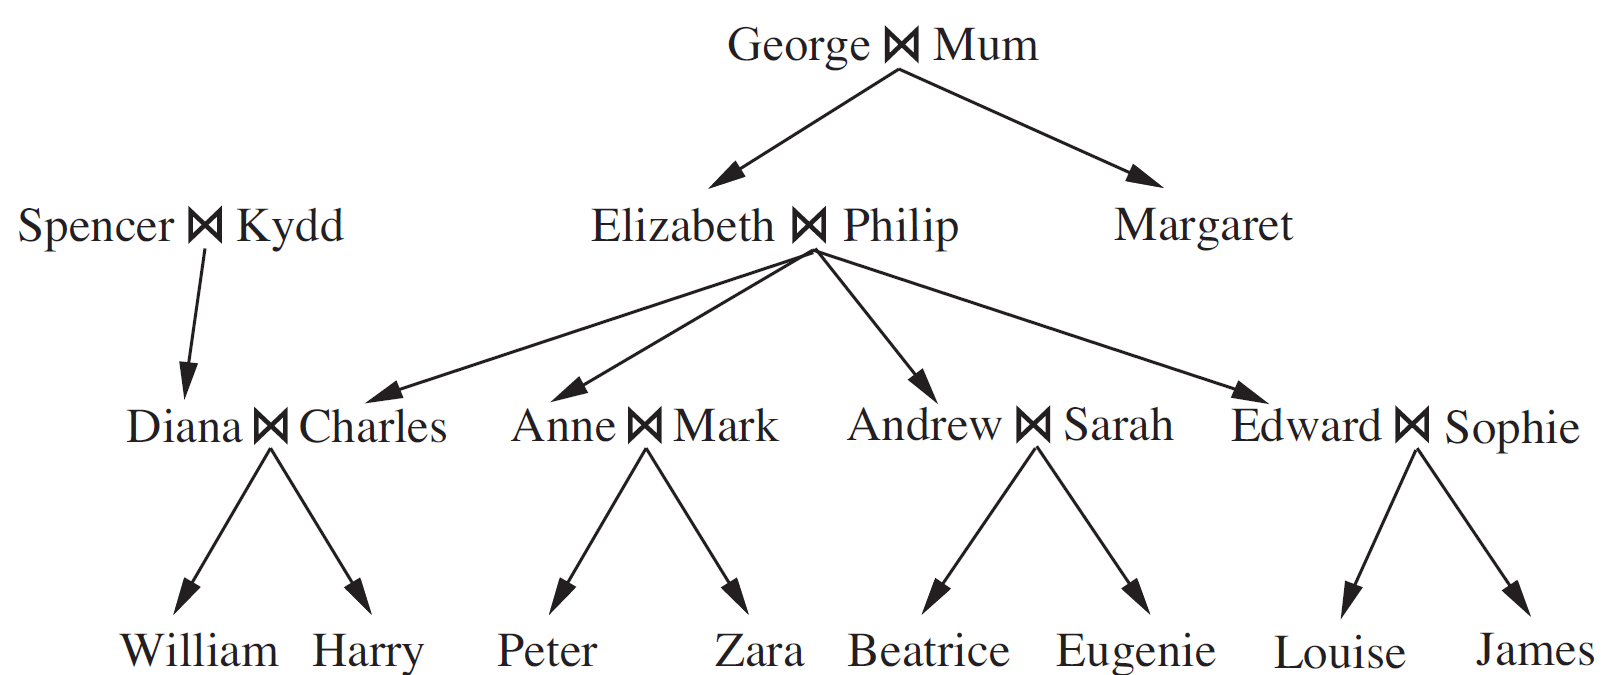
\includegraphics[width=15cm]{Pic/family}

  \label{fig:family}
  \caption{A typical family tree. The symbol $\bowtie$ connects spouses and arrows point to children.}
\end{figure}

\section{Tasks}


\begin{enumerate}
\item Please complete the \texttt{Prolog} codes. There are several tutorials in the folder and I will explain the usage of Prolog in class.
\item Write the related codes and take a screenshot of the running results in the file named \textsf{E05\_YourNumber.pdf}, and send it to \textsf{ai\_2020@foxmail.com}.

\end{enumerate}
\section{Codes}
\definecolor{mygreen}{rgb}{0,0.6,0}
\definecolor{mygray}{rgb}{0.5,0.5,0.5}
\definecolor{mymauve}{rgb}{0.58,0,0.82}
\lstset{
    backgroundcolor=\color{lightgray}, 
    basicstyle = \footnotesize,       
    breakatwhitespace = false,        
    breaklines = true,                 
    captionpos = b,                    
    commentstyle = \color{mygreen}\bfseries,
    extendedchars = false,             
    frame =shadowbox, 
    framerule=0.5pt,
    keepspaces=true,
    keywordstyle=\color{blue}\bfseries, % keyword style
    language = Prolog,                     % the language of code
    otherkeywords={string}, 
    numbers=left, 
    numbersep=5pt,
    numberstyle=\tiny\color{mygray},
    rulecolor=\color{black},         
    showspaces=false,  
    showstringspaces=false, 
    showtabs=false,    
    stepnumber=1,         
    stringstyle=\color{mymauve},        % string literal style
    tabsize=2,          
    title=\lstname                      
}
\begin{enumerate}
\item \textbf{male},\textbf{female},\textbf{child},\textbf{spouse}的实现。
注意,可能死循环的问题。
如定义规则\texttt{spouse(X, Y) :- spouse(Y, X)},没有递归终止条件。
当运用该规则查询\texttt{spouse(x, y)}时,若没有\texttt{spouse(y, x)},则会继续用改规则查询\texttt{spouse(x, y)}。
解决方法是设置递归终止到\textbf{fact}上,如\texttt{init\_spouse(y, x)}。
\begin{lstlisting}
init_male(george).
init_male(andrew).
init_male(edward).
init_male(william).
init_male(harry).
init_male(peter).
init_male(james).
init_female(spencer).
init_female(elizabeth).
init_female(margaret).
init_female(diana).
init_female(anne).
init_female(zara).
init_female(beatrice).
init_female(eugenie).
init_female(louise).
init_female(charlotte).
init_child(elizabeth, george).
init_child(margaret, george).
init_child(diana, spencer).
init_child(charles, elizabeth).
init_child(anne, elizabeth).
init_child(andrew, elizabeth).
init_child(edward, elizabeth).
init_child(william, diana).
init_child(harry, diana).
init_child(peter, anne).
init_child(zara, anne).
init_child(beatrice, andrew).
init_child(eugenie, andrew).
init_child(louise, edward).
init_child(james, edward).
init_child(charlotte, william).
init_spouse(george, mum).
init_spouse(spencer, kydd).
init_spouse(elizabeth, philip).
init_spouse(diana, charles).
init_spouse(anne, mark).
init_spouse(andrew, sarah).
init_spouse(edward, sophie).
male(X) :- init_male(X); (spouse(X, Y), init_female(Y)).
female(X) :- init_female(X); (spouse(X, Y), init_male(Y)).
child(X, Y) :- init_child(X, Y); (init_child(X, Z), spouse(Y, Z)).
spouse(X, Y) :- init_spouse(X, Y); init_spouse(Y, X).
\end{lstlisting}

\item \textbf{Grandchild},\textbf{Greatgrandparent},\textbf{Ancestor},
\textbf{Sibling},\textbf{Brother},\textbf{Sister},
\textbf{Daughter},\textbf{Son},\textbf{FirstCousin},
\textbf{BrotherInLaw},\textbf{SisterInLaw},\textbf{Aunt},\textbf{Uncle}的实现。
\begin{lstlisting}
grandchild(X, Y) :- child(X, Z), child(Z, Y).
great_grandparent(X, Y) :- child(Y, Z), child(Z, A), child(A, X).
ancestor(X, Y) :- child(Y, X); (child(Y, Z), ancestor(X, Z)).
sibling(X, Y) :- child(X, Z), child(Y, Z), X \= Y.
brother(X, Y) :- sibling(X, Y), male(X).
sister(X, Y) :- sibling(X, Y), female(X).
dauter(X, Y) :- child(X, Y), female(X).
son(X, Y) :- child(X, Y), male(X).
first_cousin(X, Y) :- grandchild(X, Z), grandchild(Y, Z), \+ sibling(X, Y), X \= Y.
brother_in_law(X, Y) :- (sister(Z, Y), spouse(X, Z));
                        (spouse(Y, Z), brother(X, Z));
                        (spouse(Y, Z), sister(A, Z), spouse(X, A)).
sister_in_law(X, Y) :- (brother(Z, Y), spouse(X, Z));
                        (spouse(Y, Z), sister(X, Z));
                        (spouse(Y, Z), brother(A, Z), spouse(X, A)).
aunt(X, Y) :- (child(Y, Z), sister(X, Z)); (child(Y, Z), sister_in_law(X, Z)).
uncle(X, Y) :- (child(Y, Z), brother(X, Z)); (child(Y, Z), brother_in_law(X, Z)).
\end{lstlisting}

\item \textbf{\emph{m}th cousin \emph{n} times removed}的实现。
\texttt{distance(X, Y, N)}考虑两种情况:一种是\texttt{X}是\texttt{Y}的祖先;
另一种是\text{X}不是\texttt{Y}的祖先,但两者有共同祖先。
\texttt{mth\_cousin\_n\_removed(X, Y, M, N)}考虑\texttt{X}和\texttt{Y}分别到共同祖先\texttt{Z}的距离,
且不存在比\texttt{Z}更小的共同距离\texttt{A},包括祖先和相等两种情况。
\begin{lstlisting}
distance(X, Y, N) :- (X = Y, N = 0);
                        (ancestor(X, Y), child(Y, Z),
                        distance(X, Z, N1), N is N1 + 1);
                        (\+ ancestor(X, Y), ancestor(Z, X), ancestor(Z, Y),
                        distance(Z, Y, N1), distance(Z, X, N2), N is N1 - N2).
mth_cousin_n_removed(X, Y, M, N) :- distance(Z, X, N1), N1 is M + 1,
                                    distance(Z, Y, N2), N2 is M + N + 1,
                                    \+ (ancestor(Z, A), (ancestor(A, X); A = X), (ancestor(A, Y); A = Y)).
\end{lstlisting}
\end{enumerate}
\section{Results}
\begin{figure}[ht]
	\centering
	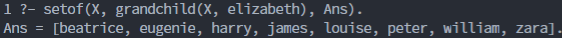
\includegraphics[width=7cm]{1.png}
	\caption{Elizabeth’s grandchildren}
	\centering
	
\includegraphics[width=7cm]{2.png}
	\caption{Diana’s brothers-in-law}
	\centering
	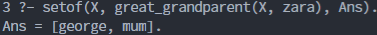
\includegraphics[width=7cm]{3.png}
	\caption{Zara’s great-grandparents}
	\centering
	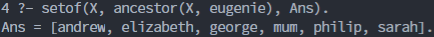
\includegraphics[width=7cm]{4.png}
	\caption{Eugenie’s ancestors}
	\centering
	
\includegraphics[width=7cm]{5.png}
	\caption{Charlotte’s first cousin once removed}
\end{figure}

%\clearpage
%\bibliography{E:/Papers/LiuLab}
%\bibliographystyle{apalike}
\end{document}
%%% Local Variables:
%%% mode: latex
%%% TeX-master: t
%%% End:
